\documentclass[border=1pt]{standalone}
% ---------------------------------------------------------------------------
% Shared style for the MOSAIC / CRYSTAL TOMM figures.
% Compile each fig_*.tex with LuaLaTeX (standalone). Sized for acmart
% "acmsmall" (TOMM): \textwidth = 13.9 cm, so every figure is drawn at
% final size and is included with width=\textwidth (no rescaling of text).
% Fonts: Libertinus Sans + Inconsolata (acmart uses Libertine + Inconsolata).
% ---------------------------------------------------------------------------
\usepackage{fontspec}
\setmainfont{LibertinusSans}[Path=fonts/, Extension=.otf,
  UprightFont=*-Regular, BoldFont=*-Bold, ItalicFont=*-Italic]
\setmonofont{Inconsolata}[Path=fonts/, Extension=.otf,
  UprightFont=*-Regular, BoldFont=*-Bold, Scale=0.98]
\usepackage{unicode-math}
\setmathfont{LibertinusMath-Regular.otf}[Path=fonts/]

\usepackage{tikz}
\usetikzlibrary{positioning,fit,calc,arrows.meta,backgrounds,
  shapes.misc,shapes.geometric,decorations.pathreplacing,patterns.meta}

% Okabe-Ito palette (colour-blind safe) + tints -------------------------------
\definecolor{oiBlue}{HTML}{0072B2}
\definecolor{oiOrange}{HTML}{E69F00}
\definecolor{oiSky}{HTML}{56B4E9}
\definecolor{oiGreen}{HTML}{009E73}
\definecolor{oiVerm}{HTML}{D55E00}
\definecolor{oiPurple}{HTML}{CC79A7}
\definecolor{oiYellow}{HTML}{F0E442}
\definecolor{ink}{HTML}{1A1A1A}
\definecolor{muted}{HTML}{5C5C5C}
\definecolor{rule}{HTML}{9A9A9A}

\definecolor{oursFill}{HTML}{DDEBF7}
\definecolor{oursDraw}{HTML}{0072B2}
\definecolor{modFill}{HTML}{FCEFD2}
\definecolor{modDraw}{HTML}{B57600}
\definecolor{upFill}{HTML}{F1F1F1}
\definecolor{upDraw}{HTML}{7D7D7D}
\definecolor{failFill}{HTML}{FBE3D6}
\definecolor{okFill}{HTML}{D9F0E8}

% Sequence colours (as in the packetization study)
\definecolor{seqSOL}{HTML}{0072B2}
\definecolor{seqTHA}{HTML}{009E73}
\definecolor{seqLON}{HTML}{CC79A7}

% Typography -----------------------------------------------------------------
\newcommand{\figfont}{\fontsize{7.5}{9}\selectfont}
\newcommand{\smallfig}{\fontsize{6.5}{7.8}\selectfont}
\newcommand{\tinyfig}{\fontsize{6}{7.2}\selectfont}
\newcommand{\code}[1]{{\ttfamily #1}}

% Provenance encoding: colour AND line style (grayscale safe) ------------------
%  ours      = new component written by us      (blue, solid 0.9 pt)
%  modified  = upstream component we patched    (orange, dashed 0.8 pt)
%  upstream  = used unmodified / third party    (grey, solid 0.45 pt)
\tikzset{
  base/.style={rectangle, rounded corners=1.6pt, align=center,
    inner xsep=3pt, inner ysep=2.6pt, font=\figfont, text=ink,
    execute at begin node={\hyphenpenalty=10000\exhyphenpenalty=10000}},
  ours/.style={base, fill=oursFill, draw=oursDraw, line width=0.9pt},
  mod/.style={base, fill=modFill, draw=modDraw, line width=0.8pt,
    dash pattern=on 2.6pt off 1.4pt},
  up/.style={base, fill=upFill, draw=upDraw, line width=0.45pt},
  dead/.style={base, fill=white, draw=oiVerm, line width=0.6pt,
    dash pattern=on 1.2pt off 1.2pt, text=oiVerm},
  note/.style={font=\smallfig, text=muted, align=left,
    execute at begin node={\hyphenpenalty=10000\exhyphenpenalty=10000}},
  lab/.style={font=\smallfig\itshape, text=muted},
  zone/.style={draw=rule, line width=0.45pt, rounded corners=3pt,
    dash pattern=on 0.6pt off 1.1pt},
  zonetitle/.style={font=\figfont\bfseries, text=ink, anchor=west,
    inner xsep=2pt, inner ysep=1pt, fill=white, xshift=2.5mm},
  flow/.style={-{Stealth[length=4pt,width=3.2pt]}, line width=0.65pt,
    draw=ink},
  dflow/.style={flow, dash pattern=on 2pt off 1.4pt},
  ctrl/.style={-{Stealth[length=3.4pt,width=2.8pt]}, line width=0.5pt,
    draw=muted},
  failflow/.style={-{Stealth[length=4pt,width=3.2pt]}, line width=0.6pt,
    draw=oiVerm, dash pattern=on 1.4pt off 1.2pt},
  stepc/.style={circle, fill=ink, text=white, inner sep=0pt,
    minimum size=8.5pt, font=\tinyfig\bfseries},
  tag/.style={font=\tinyfig\bfseries, inner sep=1pt},
}

% Legend for the provenance encoding -------------------------------------------
\newcommand{\provlegend}[1]{% #1 = anchor coordinate (north west)
  \begin{scope}[shift={(#1)}]
    \node[ours, minimum width=6mm, minimum height=2.6mm, inner sep=0pt]
      (lg1) at (0,0) {};
    \node[anchor=west, font=\smallfig] at (lg1.east) {new (this work)};
    \node[mod, minimum width=6mm, minimum height=2.6mm, inner sep=0pt]
      (lg2) at (2.6,0) {};
    \node[anchor=west, font=\smallfig] at (lg2.east) {upstream, patched by us};
    \node[up, minimum width=6mm, minimum height=2.6mm, inner sep=0pt]
      (lg3) at (6.2,0) {};
    \node[anchor=west, font=\smallfig] at (lg3.east) {upstream / third party, unmodified};
  \end{scope}}

\usepackage{array}
\newcommand{\bx}[2]{{\bfseries #1\par}\vspace{0.6pt}{\smallfig #2\par}}
\begin{document}
\figfont
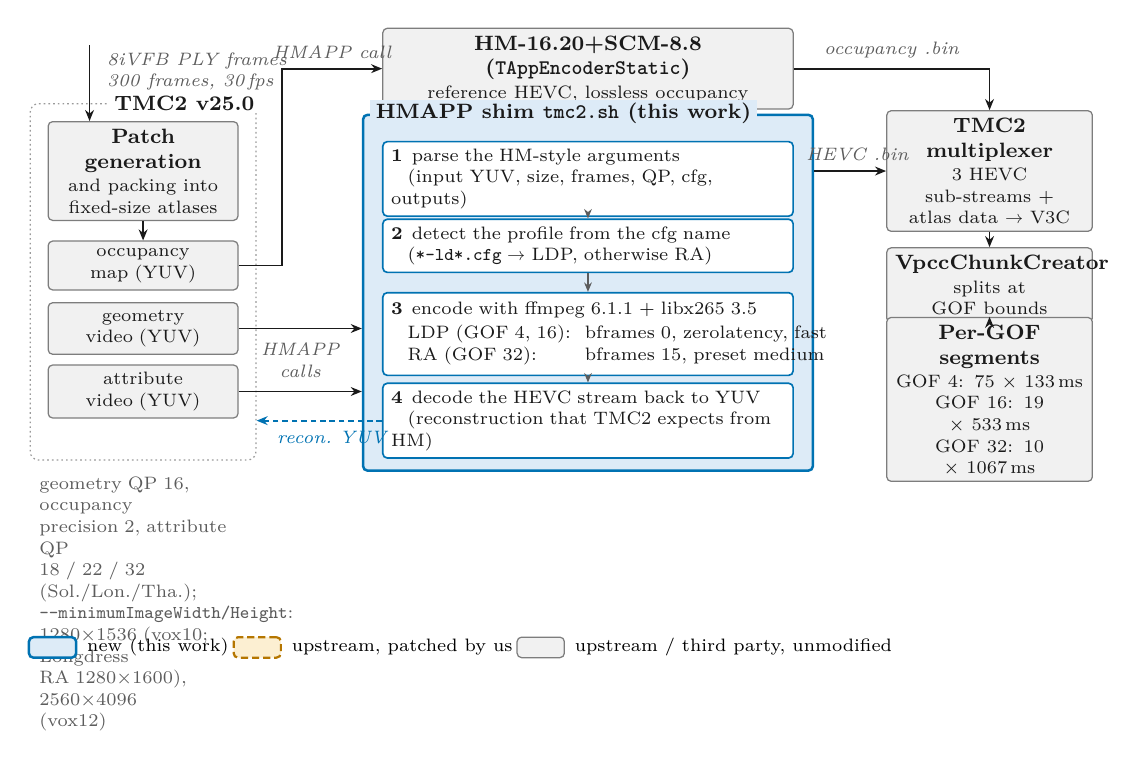
\begin{tikzpicture}[x=1cm,y=1cm]
  \tikzset{vid/.style={up, text width=2.2cm, minimum height=0.62cm, font=\smallfig},
           stepbox/.style={ours, text width=5.0cm, minimum height=0.66cm, align=left,
              font=\smallfig, fill=white, line width=0.6pt}}

  % ---------------- TMC2 front end (upstream) --------------------------------
  \node[up, text width=2.2cm, minimum height=0.95cm] (pg) at (1.3,4.05)
    {\bx{Patch generation}{and packing into\\fixed-size atlases}};
  \node[vid] (occ) at (1.3,2.85) {occupancy map (YUV)};
  \node[vid] (geo) at (1.3,2.05) {geometry video (YUV)};
  \node[vid] (att) at (1.3,1.25) {attribute video (YUV)};
  \draw[flow] (0.62,5.65) -- (0.62,0 |- pg.north);
  \node[lab, align=left, anchor=north west] at (0.72,5.68) {8iVFB PLY frames\\300 frames, 30\,fps};
  \coordinate (zlow) at (0.6,0.6);
  \draw[flow] (pg) -- (occ);
  \begin{scope}[on background layer]
    \node[zone, fit=(pg)(occ)(geo)(att)(zlow), inner sep=2.2mm] (ztmc) {};
  \end{scope}
  \node[zonetitle, anchor=east, xshift=-2.0mm] at (ztmc.north east) {TMC2 v25.0};
  \node[note, anchor=north west, text width=2.8cm] at ($(ztmc.south west)+(0,-0.08)$)
    {geometry QP 16, occupancy\\precision 2, attribute QP\\18 / 22 / 32 (Sol./Lon./Tha.);\\\code{--minimumImageWidth/Height}:\\1280×1536 (vox10; Longdress\\RA 1280×1600), 2560×4096\\(vox12)};

  % ---------------- codec dispatch -------------------------------------------
  \node[up, text width=5.0cm, minimum height=0.66cm] (hm) at (6.95,5.35)
    {\bx{HM-16.20+SCM-8.8 (\code{TAppEncoderStatic})}{reference HEVC, lossless occupancy}};

  \node[stepbox] (s1) at (6.95,3.95) {\textbf{1\,} parse the HM-style arguments\\\hspace*{6pt}(input YUV, size, frames, QP, cfg, outputs)};
  \node[stepbox] (s2) at (6.95,3.1)  {\textbf{2\,} detect the profile from the cfg name\\\hspace*{6pt}(\code{*-ld*.cfg} $\rightarrow$ LDP, otherwise RA)};
  \node[stepbox, minimum height=1.05cm] (s3) at (6.95,1.98) {\textbf{3\,} encode with ffmpeg 6.1.1 + libx265 3.5\\[1pt]
    \hspace*{6pt}\begin{tabular}{@{}l@{\hspace{5pt}}l@{}}
      LDP (GOF 4, 16): & bframes 0, zerolatency, fast\\
      RA (GOF 32):     & bframes 15, preset medium\\
    \end{tabular}};
  \node[stepbox] (s4) at (6.95,0.88) {\textbf{4\,} decode the HEVC stream back to YUV\\\hspace*{6pt}(reconstruction that TMC2 expects from HM)};
  \draw[ctrl] (s1) -- (s2); \draw[ctrl] (s2) -- (s3); \draw[ctrl] (s3) -- (s4);
  \begin{scope}[on background layer]
    \node[ours, fit=(s1)(s2)(s3)(s4), inner sep=2.4mm, fill=oursFill, yshift=0.9mm] (zshim) {};
  \end{scope}
  \node[zonetitle, fill=oursFill, xshift=-1.5mm] at (zshim.north west) {HMAPP shim \code{tmc2.sh} (this work)};

  % ---------------- arrows from TMC2 to codecs --------------------------------
  \draw[flow] (occ.east) -- ++(0.55,0) |- (hm.west) node[pos=0.75, above, lab] {HMAPP call};
  \draw[flow] (geo.east) -- (zshim.west |- geo.east);
  \draw[flow] (att.east) -- (zshim.west |- att.east);
  \node[lab, align=center] at ($(geo.east)!0.5!(zshim.west |- att.east)$) {HMAPP\\calls};

  % ---------------- back end ---------------------------------------------------
  \node[up, text width=2.4cm, minimum height=0.95cm] (mux) at (12.05,4.05)
    {\bx{TMC2 multiplexer}{3 HEVC sub-streams +\\atlas data $\rightarrow$ V3C}};
  \node[up, text width=2.4cm, minimum height=0.95cm] (chk) at (12.05,2.6)
    {\bx{VpccChunkCreator}{splits at GOF bounds}};
  \node[up, text width=2.4cm, minimum height=0.95cm] (out) at (12.05,1.15)
    {\bx{Per-GOF segments}{GOF 4: 75 × 133\,ms\\GOF 16: 19 × 533\,ms\\GOF 32: 10 × 1067\,ms}};
  \draw[flow] (hm.east) -| (mux.north) node[pos=0.25, above, lab] {occupancy .bin};
  \draw[flow] (zshim.east |- mux.west) -- (mux.west) node[pos=0.6, above, lab] {HEVC .bin};
  \draw[flow] (mux) -- (chk);
  \draw[flow] (chk) -- (out);
  % recon return
  \draw[dflow, draw=oiBlue] (s4.west) -- (ztmc.east |- s4.west)
     node[pos=0.4, below, lab, text=oiBlue] {recon.\ YUV};

  \provlegend{0.15,-2.0}
\end{tikzpicture}
\end{document}
